\section{Belægningsgrad på ortopædkirurgisk afdeling}
På ortopædkirurgisk afdeling på Aalborg Universitetshospital ses en varierende belægningsgrad for hver måned. Som tidligere nævnt i \ref{sec:kap} ønskes en fuld kapacitetsudnyttelse, hvoraf alle sengepladser ønskes at være i brug. Belægningsgraden er antallet af de anvendte disponible senge. På \figref{maxminbelaeg} ses belægningsgraden fra år $2014$ til $2015$ på ortopædkirurgisk afdeling. \cite{SDS2015}


\begin{figure}[H]
	\flushleft 
	\centering
	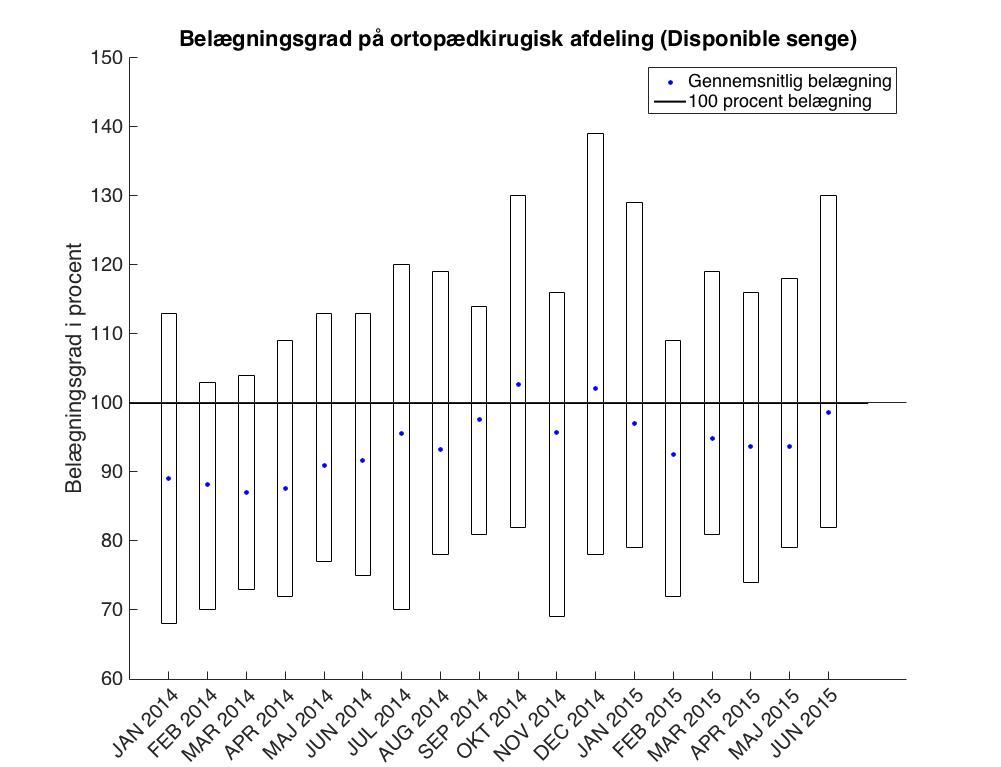
\includegraphics[scale=.45]{figures/maxminoverbelaeg.png}
	\flushleft
	\caption{\textit{Belægningsgraden på ortopædkirurgisk afdelingen på Aalborg Universitetshospital målt over $18$ måneder fra år $2014$ til $2015$. Søjlerne viser belægning ift. $100~\%$ belægning, hvortil maksimal og minimum belægning ligeledes illustreres. De blå punkter viser den gennemsnitlige belægning hver måned.}\cite{SDS2015}}
	\label{maxminbelaeg}
\end{figure}

\noindent
Det fremgår af \figref{maxminbelaeg}, at ortopædkirurgisk afdeling oplever en belægning hhv. over og under den ønskede belægning på $100~\%$. I december måned år $2014$ ses en maksimal belægning på $139~\%$ og en minimums belægning på $78~\%$. Maksimums belægning kan indikere, at der flere patienter end afdelingen er disponeret til. Dertil har afdelingen oplevet kapacitetsmangel. Minimums belægning kan indikere, at der ikke har været tilstrækkelige elektive patienter i de perioder, hvilket ligeledes medfører ubalance i kapacitetsudnyttelsen. Af \figref{maxminbelaeg} er den gennemsnitlige belægning pr. måned hyppigst under $100~\%$. Oktober og december måned i år $2014$ oplever dog en gennemsnitlig belægning over $100~\%$. Den gennemsnitlige belægning ses varierende mellem $90$ og $100~\%$, hvilket kan indikere, at afdelingen oplever kapacitetsmangel i kortvarige perioder.\cite{SDS2015} 
Det fremgår ikke af den anvendte data, hvorvidt belægningen opleves i timer eller flere døgn. Dertil skal der tages forbehold for, at det ikke er angivet om det er elektive eller akutte patienter, der udgør en belægning over $100~%$.\cite{SDS2015} 

 
For at underbygge belægningsgraden yderligere, illustrerer \figref{antaldage} antal dage pr. måned med en belægningsgrad på over $100~\%$. Denne graf er udarbejdet ud fra ortopædkirurgisk afdeling over de samme 18 måneder som \figref{maxminbelaeg}. \cite{SDS2015} 

\begin{figure}[H]
	\flushleft 
	\centering
	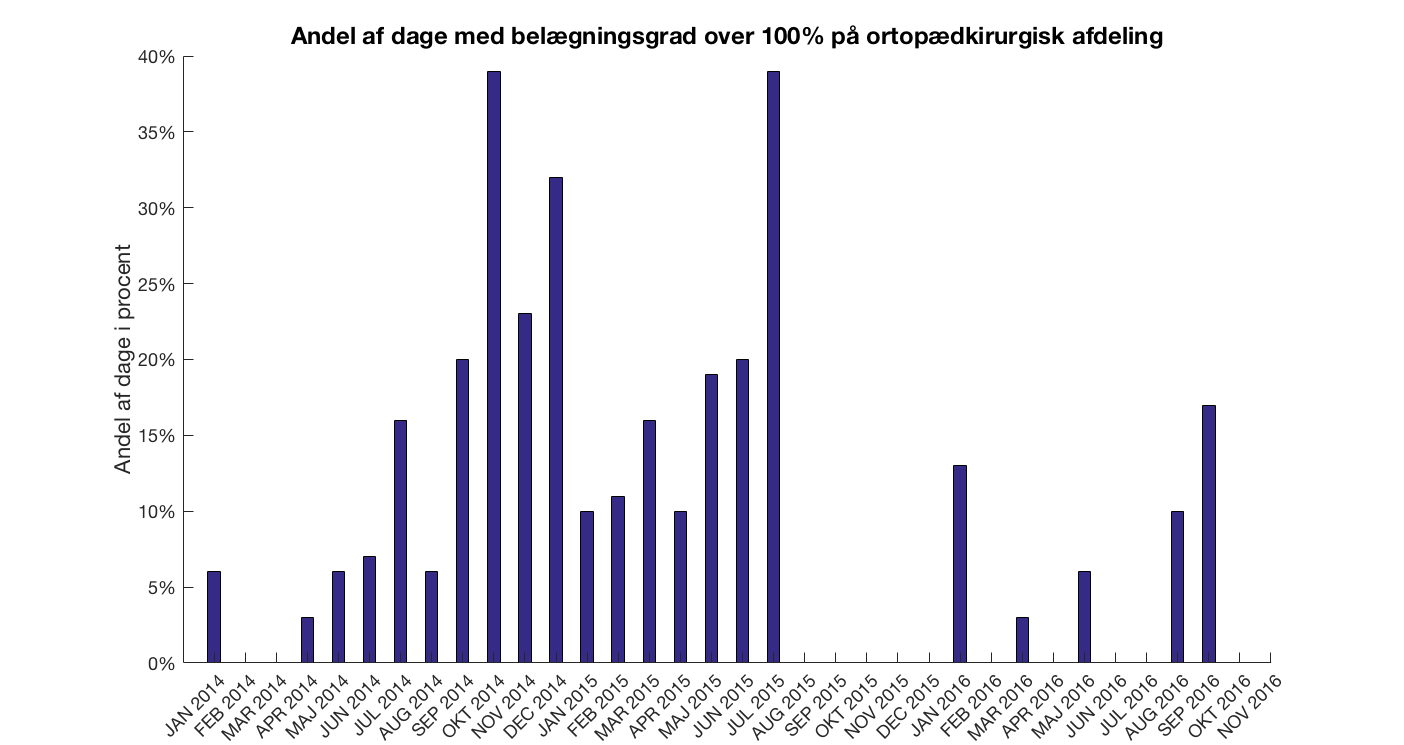
\includegraphics[scale=.4]{figures/antaldage.png}
	\flushleft
	\caption{\textit{Belægningsgrad over $100~\%$ målt i antal dage over $18$ måneder fra år $2014$ til juni $2015$ for ortopædkirugisk afdeling på Aalborg Universitetshospital.}\cite{SDS2015}}
	\label{antaldage}
\end{figure}

\noindent
Det fremgår af \figref{antaldage}, at der i oktober måned år $2014$ opleves en belægning på over $100\%$ i 19 dage, sammenlignes dette med oktober måned på \figref{maxminbelaeg} ses en belægning på $130~\%$. Dertil ses der en sammenhæng mellem antal dage med belægning over $100~\%$ og belægningsgraden over $100~\%$. 




I oktober måned år $2014$ fremgår det af \figref{antaldage} at der er 19 dage med 


Der ses i oktober måned år $2014$ på \figref{maxminbelaeg} en belægningsgrad på $130~\%$, hvor der ses på \figref{antaldage} 


opleves der i samme måned en belægning på $130~\%$. Derudover ses der en sammenhæng mellem de to figurer, hvor søjlerne i \figref{antaldage} følger belægning over $100~\%$ i \figref{maxminbelaeg}. 






Det ses i \figref{maxminbelaeg}, at der i oktober måned år 2014 opleves en belægning på $130 \%$, hvilket kan opholdes mod de 19 dage. 

Det vides dog ikke, hvorvidt der er tale om én ekstra eller flere patienter, der udgør en belægningsgrad på over $100 \%$, samt hvor længe patienterne er indlagt på afdelingen. Det ses i \figref{maxminbelaeg}, at der i oktober måned år 2014 opleves en belægning på $130 \%$, hvilket kan opholdes mod de 19 dage. Det skal understreges, at begge grafer er angivet i måneder, og det er derfor uvist om, hvor mange patienter, der er indlagt pr. dag. Derudover er figurerne, \figref{maxminbelaeg} og \figref{antaldage}, udarbejdet over 18 måneder, hvilket angiveligt ikke er en repræsentativ periode for at konkludere et reelt problem på afdelingen. Dertil vides det ikke om belægningsgraden over $100 \%$ opleves som værende et problem på ortopædkirurgisk afdeling på Aalborg Universitetshospital eller om det blot er et strukturerings problem.  \fxnote{Problemet virker så opfattende - vi underskylder for meget.}